% next line is used by my TeXShop environment; do not remove, Doaitse
% !TEX root = ../ldta_tool_challenge.tex
\newcommand{\doaitse}[1]{\marginpar{\textcolor{red}{\textbf{Doaitse:}#1}}}
\newcommand{\marcos}[1]{\marginpar{\textcolor{red}{\textbf{Marcos:}#1}}}

\newpage

\lstdefinelanguage{haskell}{
keywords={module, where, let, in, case, of, proc, rec, do, if, then, else, data, type, deriving},
sensitive=true
}
\newcommand{\haskellsize}{\fontsize{9pt}{9pt}}
\lstnewenvironment{haskell} 
{\lstset{language={haskell}}\haskellsize}{}
\lstset{
      basicstyle=\small\ttfamily,
      flexiblecolumns=false,
      tabsize=4,
      fontadjust= true,
      lineskip=0.7pt,
      aboveskip=\baselineskip,
      belowskip=\baselineskip,
      frame=tb,
      showspaces=false,
      showtabs=false,
      framerule=0.5pt,
      framexleftmargin=0.2cm,
      numbers=none,
      basewidth={0.5em,0.45em},
      literate={+}{{$+$}}1 {/}{{$/$}}1 {*}{{$*$}}1 {=}{{$=$}}1
               {>}{{$>$}}1 {<}{{$<$}}1  {\\}{{$\lambda$}}1
               {\\\\}{{\char`\\\char`\\}}1
               {->}{{$\rightarrow$}}2 {>=}{{$\geq$}}2 {<-}{{$\leftarrow$}}2
               {<=}{{$\leq$}}2 {=>}{{$\Rightarrow$}}2 
	       {<<<}{{$\lll$}}2 {>>>}{{$\ggg$}}2 {-<}{{$\prec{}$}}2
               {>>}{{>>}}2 {>>=}{{>>=}}2 {+>>}{{+>>}}2 {<|>}2
	       {|}{{$\mid$}}1 {iI}{{$\llfloor$}}1 {Ii}{{$\rrfloor$}}1
	       {undefined}{{$\perp$}}1 {\\\$}{{\$}}1 
       }
\newcommand\texthaskell[1]{{\lstinline[language={haskell}]{#1}}}
\newcommand\texthaskellF[1]{{\haskellsize\lstinline[language={haskell}]{#1}}}


\section{CoCoCo: Compositional Compiler Construction in Haskell}

\subsection{Introduction}

CoCoCo\footnote{\url{http://www.cs.uu.nl/wiki/bin/view/Center/CoCoCo}} is a set of libraries and tools in the form of a collection of embedded domain specific languages (EDSL) for constructing extensible compilers,
where compilers can be composed out of \emph{separately compiled}  
language-definition fragments. The Haskell type system  not only checks the expressions inside a component, but also the mutual consistency of a collection of components. Our approach builds on:
\begin{itemize}
%\item the introduction of typed abstract syntax \cite{BaSw02}
\item the introduction of a naming structure which makes it possible to represent mutually dependent 
recursive structures such as context free grammars and to inspect and manipulate such structures in a type-safe way \cite{BSV09}
\item the description of typed grammar fragments as first class Haskell values \cite{VSD12}, and the typed Left-Corner Transform to remove left-recursion \cite{BSV09b}
\item the possibility to construct a self-analysing, error correcting parser on the fly \cite{Swie2000,Swierstra08}
\item the possibility to deal with attribute grammars as first class  Haskell values, which can be transformed, composed and finally evaluated \cite{Viera:Attribute-Grammars,UU-CS-2011-028,VSM12}.
\end{itemize}

 

\subsection{Architecture and Parsing}

Using our combinator library\footnote{\url{http://hackage.haskell.org/package/murder}} \cite{VSD12} we describe  the concrete syntax of each language fragment as a Haskell value.
A fragment of the {\em code constructing the CFG} of the initial language L1 is given in Figure~\ref{fig:gram} in which we recognise the underlying left-recursive context free grammar.
\begin{figure}[th]
\begin{center}
\begin{haskell}
l1 sf = proc _ -> do
   rec modul  <- addNT -< ...
       ...
       exp    <- addNT -< iI sexp   Ii <|> 
                          iI (pEExp     sf) exp  "=" sexp   Ii <|> ...
       sexp   <- addNT -< iI signed Ii <|> 
                          iI (pPlusExp  sf) sexp "+" signed Ii <|> ...
       signed <- addNT -< iI term   Ii <|> 
                          iI (pNegExp   sf) "-" term Ii <|> ... 
       term   <- addNT -< iI factor Ii <|> 
                          iI (pTimesExp sf) term "*" factor Ii <|> ...
       factor <- addNT -< iI (pIdExp    sf) ident Ii <|>  
                          iI (pIntExp   sf) int   Ii <|> ...
       ...
   exportNTs -< exportList modul \$ export cs_Expression exp ...
\end{haskell}
\vspace{-15pt}
\caption{Fragment of the concrete syntax specification of L1}
\label{fig:gram}
\end{center}
\end{figure}
Each grammar fragment consists of a sequence of grammar transformations expressed in Haskell's arrow syntax \cite{507664}, each of the form \texthaskell{output <- transformation -< input}. Each transformation updates the implicitly maintained grammar description.
New non-terminals (syntactic category) of the CFG are introduced using  \texthaskell{addNT} transformations, which take as input an initial set of productions for that non-terminal and returns a value which may be used in other transformations to refer to this new non-terminal.  Each right hand side of a production (alternative) is expressed in so-called \emph{applicative style} \cite{McB07},
using idiomatic brackets \texthaskell{iI} and \texthaskell{Ii} to delineate the list of components constituting an alternative. Note that the resulting notation closely resembles a similar description in a dedicated language.  The Haskell type of an element determines the r\^ole the element plays in the parsing process and the final semantics of the alternative: \texthaskell{String} values are e.g. interpreted as keywords to be recognised, and carry no semantic value of their own, functions do not require any parsing (i.e. correspond to the empty token sequence) but carry a value which is the function value itself, and non-terminal references both have a parsing effect  and construct a semantic value.
Alternatives for the same non-terminal are combined with the \texthaskell{<|>} (choice) operator.

The semantics of an abstract syntax tree is a Haskell function mapping inherited to synthesised attributes; attribute grammar evaluation can be performed without explicit scheduling, since we implicitly make use of Haskell's lazy evaluation. In case attributes have a circular definition we take the least fixed-point semantics, which usually leads to an infinite structure. Fortunately this is no problem with Haskell as a host language.
The parameter \texthaskell{sf} in Figure~\ref{fig:gram}  contains the ``semantics of the language''; it is a record containing the semantics for all the productions, from which expressions like \texthaskell{pEExp sf} elect the appropriate element. Such functions compute the semantics of the recognised left hand side non-terminal of a production in terms of the semantics associated with the children of that production, which themselves are  functions mapping inherited to synthesised attributes.


Grammars defined in this way are \emph{extensible}, since further transformations may be applied to the grammar under construction in other modules.  
Each grammar exports (with \texthaskell{exportNTs}) its starting point (e.g. \texthaskell{modul}) and a table  of
\emph{exported non-terminals}, each consisting of a label (by convention of  the
form \texthaskell{cs_...}) and a reference to the current definition of that non-terminal, again a plain Haskell value which can be used and modified in future extensions.
Figure~\ref{fig:gram2} contains a fragment of the definition of L2, 
which extends the L1 grammar with a \textoberon{CASE} statement.
\begin{figure}[th]
\begin{center}
\begin{haskell}
l2 sf = proc imported -> do
     let statement = getNT cs_Statement     imported 
     let exp       = getNT cs_Expression    imported 
     let mbelse    = getNT cs_MaybeElseStmt imported 
     ...
     rec addProds -< (statement,iI(pCaseStmt sf) "CASE" exp "OF" 
                                                 c cs mbelse "END"Ii)
     ...
     exportNTs -< imported
\end{haskell} 
\vspace{-15pt}
\caption{Fragment of the grammar extension L2}
\label{fig:gram2}
\end{center}
\end{figure}
We start by retrieving references to all non-terminals which are to be extended or used (using \texthaskell{getNT}) from the \texthaskell{imported} non-terminals.
We add new productions to existing non-terminals with \texthaskell{addProds}; this does not lead to references to new non-terminals.
New non-terminals can stikk be introduced as well using \texthaskell{addNT}.
The Haskell type-system ensures that 
the \texthaskell{imported} list indeed contains a table with entries \texthaskell{cs_Statement}, 
\texthaskell{cs_Expression} and \texthaskell{cs_MaybeElseStmt}, 
and that the types of these non-terminals coincide with their use in the semantic functions of
the extensions.

The definition in Figure~\ref{fig:gram2} may look a bit verbose, caused by  the interface having been made explicit. 
Using some Template Haskell this can  easily be overcome.

The architecture of our implementation of Oberon0 is given in Figure~\ref{fig:modules};
boxes represent Haskell modules and arrows are \texthaskell{import} relations, where every module can be compiled separately and results in a set of normal Haskell value definitions. 
The design is incremental:  rows corresponds to syntactic extensions (language levels) and
 columns corresponds to semantic extensions (tasks);
each artifact in the challenge corresponds to a dashed box surrounding the modules involved in it.
\begin{figure}[th]
\begin{center}
	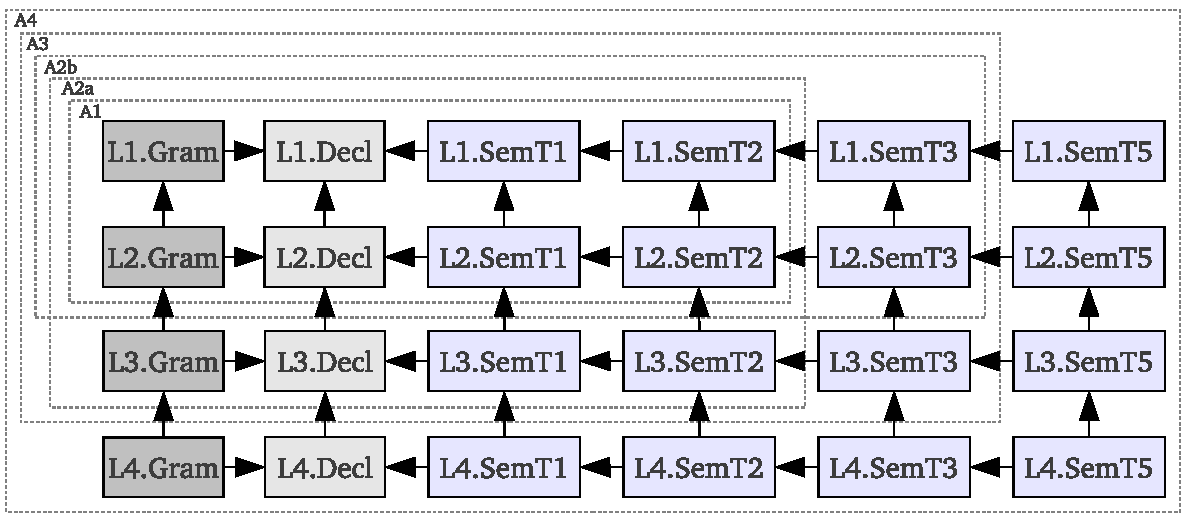
\includegraphics[scale=0.65]{cococo/modules.pdf}
\caption{Architecture of Oberon0}
\label{fig:modules}
\end{center}
\end{figure}
For each language level \texthaskell{L1} to \texthaskell{L4}: 
\begin{itemize}
	\item  \texthaskell{Gram} modules contain  syntax definition (i.e. \texthaskell{L1.Gram} contains \texthaskell{l1}, \texthaskell{L2.Gram} contains \texthaskell{l2}, etc.)
	\item \texthaskell{Decl} modules contain the definition of the type of the semantics' record, and thus the interface to the abstract syntax of the language at hand
	\item \texthaskell{Sem} modules implement the semantics of each task in the form of rules which construct an attribute grammar
\end{itemize}

To build a compiler, e.g. Artifact 4 (Figure~\ref{fig:A4}), we import the syntax fragments (\texthaskell{l1}, \texthaskell{l2}, 
\texthaskell{l3} and \texthaskell{l4} 
from \texthaskell{L4.Gram}) and their respective semantics (\texthaskell{l1t4}, 
\texthaskell{l2t4}, \texthaskell{l3t4} and \texthaskell{l4t4} from \texthaskell{L4.Sem}), 
combine them and build the compiler in the form of a parser which calls semantic functions.
\begin{figure}[th]
\begin{minipage}[b]{0.5\linewidth}
\begin{center}
	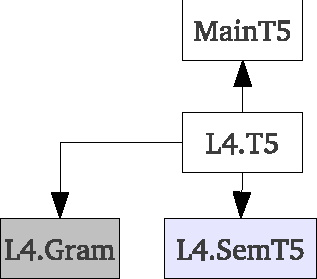
\includegraphics[scale=0.6]{cococo/main.pdf}
\caption{Architecture of Artifact 4}
\label{fig:A4}
\end{center}
\end{minipage}
\hspace{0.2cm}
\begin{minipage}[b]{0.5\linewidth}
\begin{haskell}
gl4t5 = closeGram \$ emptyGram +>> 
                    l1 l1t5   +>> 
                    l2 l2t5   +>> 
                    l3 l3t5   +>> 
                    l4 l4t5

pA4 = (parse . generate kws) gl4t5
\end{haskell}
\vspace{-15pt}
\caption{A Parser for Artifact 4}
\label{fig:pA4}
\end{minipage}
\hspace{0.5cm}
\end{figure}
In Figure~\ref{fig:pA4} we show how the parser of Artifact 4 is generated. 
The left-associative operator (\texthaskell{+>>}) composes an initial grammar with an extension;
we start with an empty grammar (\texthaskell{emptyGram}) and extend it with the different language fragments.
The function \texthaskell{closeGram} closes the constructed grammar and applies the \emph{left-corner transform} in order to remove potential left-recursion; 
as a consequence straightforward combinator-based top-down parsing techniques can be used in building the parser. 
Then \texthaskell{generate kws} generates a parser integrated with the semantics for the language starting from the first non-terminal,
where the list \texthaskell{kws} is a list of keywords extracted from the grammar description. 
This takes care of the problem how to make sure that some identifiers in earlier challenges may become keywords in later challenges. 
The function \texthaskell{parse} performs the parse of the input program and computes the meaning of that program.
In the actual implementation of Oberon0 we generate scanner-less uu-parsinglib\footnote{\url{http://hackage.haskell.org/package/uu-parsinglib}} parsers;
%our library also provides  support for uulib\footnote{\url{http://hackage.haskell.org/package/uulib}} based parsers.





\subsection{Aspect Oriented Semantics}
The semantics of Oberon0 were implemented using the
AspectAG\footnote{\url{http://hackage.haskell.org/package/AspectAG}}
\cite{Viera:Attribute-Grammars} embedding of attribute grammars in Haskell.  
In order to be able to redefine attributes or to add new attributes later, 
it encodes the lists of inherited and synthesized attributes of a
non-terminal as an HList-encoded \cite{KLS04} value; each attribute is associated with a unique type which is used as an index in such a ``list''. The lookup process is performed by the Haskell class mechanism.  
In this way the \emph{closure test} of the attribute grammar
(each attribute has a single definition) is implicitly realised by the Haskell compiler when building the right instances of the classes.
Thus, attribute grammar fragments can be individually
type-checked, compiled, distributed and composed to construct a
compiler.  

\subsubsection{Name analysis}
Error messages produced by the name analysis are collected in 
a synthesized attribute called \texthaskell{serr}\footnote{By convention we use the prefix \texthaskell{i} and \texthaskell{s} for inherited and synthesized attributes, respectively.}.
The default behaviour of this attribute for most of the productions is to combine (append) the errors produced by 
the children of the production.
This behaviour is captured by the  function \texthaskell{use} from the AspectAG library, 
which takes as arguments the label of the attribute to be defined (\texthaskell{serr}), 
the Haskell list of non-terminals (labels) for which the attribute is defined (\texthaskell{serrNTs}), 
an operator for combining the attribute values (\texthaskell{++}), 
and a unit value to be used when none of the children has such an attribute (\texthaskell{[]::String}).
\begin{haskell}
serrRule = use serr serrNTs (++) ([] :: [String]) 
\end{haskell}
When a new name is defined we check for multiple declarations and at
name uses we check for incorrect uses or uses of undefined identifiers, producing error messages when appropriate.
The code below shows the definition of \texthaskell{serr} for the use of an identifier
represented by a production
\texthaskell{IdExp}, which has a child named \texthaskell{ch_id_IdExp} of type \texthaskell{(DTerm String)}\footnote{\texthaskell{DTerm a} is the type used by murder to represent \emph{attributed terminals} (i.e. identifiers, values); it encodes the value (\texthaskell{value}) and position in the source code (\texthaskell{pos}) of the terminal.}.
\begin{haskell}
serrIdExp = syn serr \$ do 
    lhs <- at lhs
    nm  <- at ch_id_IdExp
    return \$ checkName nm (lhs # ienv) ["Var","Cst"] "an expression"
\end{haskell}
With the (plain Haskell) function \texthaskell{checkName} we lookup the name (\texthaskell{nm}) 
in the symbol table (inherited attribute \texthaskell{ienv} coming from the left-hand side)
and, if it is defined, we verify that the name represents either a variable (\texthaskell{"Var"}) 
or a constant (\texthaskell{"Cst"}) and generate  a proper error message if not.

The symbol table is implemented by the pair of attributes \texthaskell{senv} and \texthaskell{ienv}.
The synthesized attribute \texthaskell{senv} collects the information from the name declarations
and the inherited attribute \texthaskell{ienv} distributes this information through the tree.

In order to perform the name analysis, the type of the symbol table could have been 
\texthaskell{Map String NameDef}, which is a map from names to values of type \texthaskell{NameDef} 
representing information about the bound name. However, since we want to use the same symbol table
for future extensions, we keep the type ``non-closed'' by using a list-like structure:
\begin{haskell}
data SymbolInfo b a = SI b a
type NMap a = Map String (SymbolInfo NameDef a)
\end{haskell}
For the current  task the symbol table includes values of type \texthaskell{NMap a},
parametric in \texthaskell{a}, the ``the rest of the information we might want to store for this symbol''.
In the example below, for declarations of constants, the table consists of a map from the introduced name 
to a \texthaskell{SymbolInfo} which includes the information needed by the name analysis (constructed using \texthaskell{cstDef})
and some other (yet unknown) information, which is represented by the argument the rule receives:
\begin{haskell}
senvCstDecl r = syn senv \$ do  
                  nm <- at ch_id_CstDecl
                  return \$ Map.singleton (value nm) 
                                         (SI (cstDef \$ pos nm) r)
\end{haskell}
Similarly to how we used \texthaskell{use} for the default cases of synthesized attributes,
we capture the behaviour of distributing an inherited attribute to the children of a production
with the function \texthaskell{copy}:
\begin{haskell}
ienvRule _ = copy ienv ienvNTs 
\end{haskell}

The various aspects introduced by the attributes are combined using the function \texthaskell{ext}:
\begin{haskell}
aspCstDecl r = senvCstDecl r `ext` ienvCstDecl r `ext` 
               serrCstDecl   `ext` T1.aspCstDecl
\end{haskell}
In this case, for the production \texthaskell{CstDecl}, we extend \texthaskell{T1.aspCstDecl}, 
which is imported from \texthaskell{L1.SemT1} and includes the pretty-printing attribute,
with the attributes implementing the name analysis task (\texthaskell{serr}, \texthaskell{ienv} and \texthaskell{senv}).

Once the attributes definitions are composed, the semantic functions for the productions may be computed using the function \texthaskell{knit}.
For example, the semantic function of the production \texthaskell{CstDecl} in the case of \texthaskell{L1.SemT2} 
is \texthaskell{knit (aspCstDecl ())}. The use of \texthaskell{()} (unit) here is just to ``close the symbol table'',
since the rest of the information is not needed by the rules of Task 2.

\subsubsection{Type checking}

Type error messages are collected in the synthesized attribute \texthaskell{sterr}.
For type checking we extend the symbol table with the type information (\texthaskell{TInfo}) of the declared names.
This is done by \emph{updating} the value of the attribute \texthaskell{senv} with the function \texthaskell{synupdM}, 
which is similar to \texthaskell{syn} but redefines it making use of its current definition. 
In the following example we update the symbol table information for the production \texthaskell{VarDecl},
where \texthaskell{sty} is an attribute defined for expressions and types, computing their type information:
\begin{haskell}
senvVarDecl' r = synupdM senv \$ do 
        typ <- at ch_typ_VarDecl
        return \$ Map.map (\ (SI nd _) -> (SI nd \$ SI (typ # sty) r))
\end{haskell}
The previous definition of the type information is just ignored and only used to indicate the type of the symbol table.
Thus, thanks to lazy evaluation, when extending the aspects of Task 2 we only need to pass  an undefined value of type \texthaskell{SymbolInfo TInfo a}, 
where \texthaskell{a} is the type of the new rest of the symbol table (for future extensions):
\begin{haskell}
undTInfo :: a -> SymbolInfo TInfo a
undTInfo = const undefined

aspVarDecl r = (senvVarDecl' r) `ext` sterrRule `ext` 
               (T2.aspVarDecl \$ undTInfo r)
\end{haskell}

To represent type information we have to deal again with the lack of open data types in Haskell,
since we want to keep some specific information for each of the types of the extensible type system we are implementing, and we have decided to resort to the use of Haskell's \texthaskell{Dynamic} type. 
A \texthaskell{TInfo}, with the information of a certain type, consists of:
the representation \texthaskell{trep} of the given type, encapsulated as a \texthaskell{Dynamic} value, 
a \texthaskell{String} with its pretty-printing (\texthaskell{tshow}), 
and a function \texthaskell{teq} that, given another type information indicates if the actual type is compatible
with the given one.
\begin{haskell}
data TInfo = TInfo { trep  :: Dynamic
                   , tshow :: String 
                   , teq   :: (TInfo -> Bool) } 
\end{haskell}
%\doaitse{we could make this a Maybe to represent unity?}
The main task we perform during type checking is to verify whether the 
actual type of an expression is compatible with the type expected by its context.
For example if the condition of an \textoberon{IF} statement has type \textoberon{BOOLEAN}.
\begin{haskell}
check pos expected got 
  = if (teq expected got) || (teq got unkTy) || (teq expected unkTy)
    then []
    else [show pos ++ ": Type error. Expected " ++ show expected ++
          ", but got " ++ show got]  
\end{haskell}
If either the expected or the obtained type is unknown (\texthaskell{unkTy}) 
we do not report a type error, because unknown types are generated by 
errors that have been already detected by the name analysis process.

A very simple case of type information is the elementary type \textoberon{BOOLEAN},
where we do not provide any extra information than the type itself.
Thus, the type representation is implemented with a singleton type \texthaskell{BoolType}.
\begin{haskell}
data BoolType = BoolType 

boolTy = let d   = toDyn BoolType
             bEq = (==) (dynTypeRep d) . dynTypeRep . trep . baseType   
         in  TInfo d "BOOLEAN" bEq	        
\end{haskell}
To construct the corresponding \texthaskell{TInfo} we convert a \texthaskell{BoolType} value 
into a \texthaskell{Dynamic} with the function \texthaskell{toDyn}.
A type is compatible with \textoberon{BOOLEAN} if its base type\footnote{In case of a user type, the type it denotes.}
is also \textoberon{BOOLEAN}, i.e. is compatible if both types are represented with \texthaskell{BoolType} values.
With the function \texthaskell{dynTypeRep} we extract a concrete representation of the type of the value inside a \texthaskell{Dynamic} 
that provides support for equality.

There exist some other cases were a more involved type representation is needed.
For example, in the case of \textoberon{ARRAY} we include the type information of its elements 
and the length of the array, if it can be statically computed.
\begin{haskell}
data ArrType = ArrType (Maybe Int) TInfo 
\end{haskell}
Then, by using the type-safe cast function \texthaskell{fromDynamic} we can get access to 
this information provided the dynamic typed value represents an array.
Thus, when trying to index a variable, we can for example check if the index is out of range;
in case the cast does not succeed we  indicate that the variable we are trying to access is not an array:
\begin{haskell}
checkSelArray pos ty ind
  = case (fromDynamic . trep . baseType) ty of
     Just (ArrType l _) -> checkIndex pos ind l
     _                  -> [show pos ++ 
                            ": Accessed variable is not an array"] 
\end{haskell}
We use the same technique to keep information about the fields of a \textoberon{RECORD}
and the parameters of a \textoberon{PROCEDURE}.

\subsubsection{Source-to-source transformation}

In \cite{VS12} we extended AspectAG with an \texthaskell{agMacro} combinator that enables us
to define the attribute computations of a new production in terms of the attribute computations of existing productions.
We defined the semantics of the extensions of the language level L2 using this macro mechanism.
The \textoberon{FOR}-loop is implemented as a \textoberon{WHILE}-loop 
and the \textoberon{CASE} statement is defined in terms of an \textoberon{IF}-\textoberon{ELSIF}-\textoberon{ELSE} cascade.
In the cases were specialized behaviour is needed, like for example pretty-printing, it is still possible to redefine the attributes
involved on these aspects. As such, our mechanism is much more expressive than conventional macro mechanisms, which only perform a structure transformation. Using the library we get Task~4 almost for free.

Our approach is not very suitable for some other kind of source-to-source transformations like optimizations,
because we do not represent the AST with values (if we want to keep the AST extensible) and
we (still) do not have higher-order attributes.
Although a possible approach is to generate an AST of a fixed core language and perform 
the optimizations in this language.

\subsubsection{Code generation}

We generate the C abstract syntax representation provided by the package language-c\footnote{http://hackage.haskell.org/package/language-c}.
This package also includes a pretty-printing function for the abstract syntax.

Since ANSI C does not include nested functions  we have to lift  all the procedures, 
types and constants definitions to top-level when generating the C code required by the challenge (note that  the lifting as specified is trivial, 
since the exercise does not require bindings to be lifted properly).
In order to avoid name clashes with C keywords or due to the lifting process, we rename every identifier to make it unique.  
New names are composed by: a character \texthaskell{'_'} (assuring no clashes with C keywords),
the path (module and procedure names) to the scope were the name is defined and the actual name. 
Thus, if we have the following Oberon0 program:
\begin{oberon0}
MODULE A;
  VAR B_C : INTEGER;
  PROCEDURE B;
    PROCEDURE C;
    END C
  END B
END A.
\end{oberon0}
The names are mapped: the variable name \texthaskell{B_C} to \texthaskell{A_B_C},
the procedure name \texthaskell{B} to \texthaskell{A_B} and
the procedure name \texthaskell{C} to \texthaskell{A_1B_C}.
When prefixing with procedure names we add the number 1 at the beginning,
to make this name an invalid Oberon identifier, in order to avoid new clashes
like the one we could have had between the new names for \texthaskell{B_C}
and \texthaskell{C}.

To implement the renaming we extend the symbol table with the name mapping.

\subsection{Artifacts}

In Table~\ref{table:locs} we show the complexity (in lines of code) of our implementation of the compiler,
disaggregated into the different tasks and language levels.
The \emph{Common} column includes the \texthaskell{Gram} and \texthaskell{Decl} files,
while the \emph{Common} row includes some code used by the \texthaskell{Main} modules.
\begin{table}\centering
\begin{tabular}{ | c || c | c | c | c | c | c | }
  \hline                        
  \emph{Lang. / Task} & \emph{Common} & \emph{T1} & \emph{T2} & \emph{T3} & \emph{T5} & \emph{Total} \\
  \hline                        
  \hline                        
  \emph{Common} & - & 42 & 14 & - & 23 & 79  \\
  \hline                        
  \emph{L1} & 128 & 156 & 147 & 220 & 228 & 879  \\
  \hline  
  \emph{L2} & 187 & 98 & 69 & 65 & 56 & 475  \\
  \hline  
  \emph{L3} & 94 & 75 & 75 & 134 & 145 & 523  \\
  \hline 
  \emph{L4} & 48 & 67 & 56 & 197 & 95 & 463  \\
  \hline 
  \emph{Total} & 457 & 438 & 361 & 616 & 547 & 2419  \\
  \hline 
\end{tabular}
\caption{Code sizes (in lines of code) of the components of the compiler}
\label{table:locs}
\end{table}

The code includes 26 lines of Template Haskell, calling functions defined in the libraries to avoid some boilerplate.

We have implemented all the combinations from L1-T1 to L4-T5, including the artifacts proposed by the challenge.

%\subsection{Observations}


\subsection{Conclusions}

The most important aspect of our approach is the possibility to construct a compiler 
out of a collection of pre-compiled, statically type-checked, possibly mutually dependent
language-definition fragments written in Haskell, but with a DSL taste.

When looking at all the aspects we have covered we can conclude that we managed to find solutions for all aspects of the problems; 
we were rescued by the fact that we could always fall back to plain Haskell, 
in case our libraries were not providing a standard solution for the problem at hand. 
We have seen such solutions for dealing with flexible symbol tables, generating new identifiers and types.

We mention again that our implementation is quite verbose, since each module contains quite some code ``describing its interface'' in the collection of co-operating modules. 
This is the price we have to pay for getting the extreme degree of flexibility we are providing. 
By collapse the modules the amount of linking information shrinks considerably.
Other option to reduce verbosity is to use uuagc to generate AspectAG code \cite{VSM12}.

Another cause of the verbosity is that we have not used the system itself or Template Haskell to capture common patterns. 
We have chosen to reveal the underlying mechanisms, the role of the type system, the full flexibility provided, 
and have left open the possibility for further extensions.

The lack of open data types in Haskell makes it hard to implement AST transformations in extensible languages using our technique.
Semantic macros solve some of these problems. A possible approach is to use our technique to implement the front-end of a compiler,
translating to a core fixed language, and then use other more traditional approaches (like uuagc) to implement the back-end.

